\scanpage{20}
\uline{Locally tame space} \deleted{locally compact} \inserted{ind-tame} spaces whose topology is \deleted{locally compact} Hausdorff, and every point admits a \uline{neighborhood} which is \deleted{\unsure{space|compact}} tame (so the space is locally compact), and every point admits a fundamental system of tame neighborhoods, and the compact subsets are the subsets contained in a tame subset --- which therefore form a cofinal antifilter: that of compact subsets.

For example, by $(M10)$ $R$ is a $\mathrm{loc}^{\mathrm t}$ tame space, so the $R^I$ too.

The locally tame spaces \deleted{$\unsure{f}\ \operatorname{Esploc}_{\mathcal M_*}$} form a full subcategory $\operatorname{Esploc}_{\mathcal M_*}$ of $\underrightarrow{\operatorname{Esp}}_{\mathcal M_*}$, stable under finite $\varprojlim$.

\margin{Say that a compact and \deleted{closed} subset of a tame space is tame.}
\margin{\deleted{\unsure{locally}}}
\figure{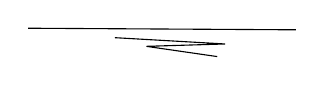
\begin{tikzpicture}\draw (0,0)--(3.4,-.02);\draw (1.1,-.12)--(2.5,-.2)--(1.5,-.23)--(2.4,-.36);\end{tikzpicture}}
\mspage{19}
